% !TEX root = ../EjsS Manual.tex

\chapter{Converting from Java to Javascript}\label{chapter:JavatoJS}

\begin{quote}
Everything must change so that everything can remain the same  {\em Giuseppe di Lampedusa in `The Leopard'}
\end{quote}

In this chapter, we go through the process of porting an existing Java simulation created with \ejs\ into an equivalent Javascript simulation. The architecture of \ejs\ shows how this can be easily done, the \lit{HtmlView} being the only part that needs to be re-created from scratch. 

% ------------------------
    \section{Porting a simulation}\label{section:04Loading}
% ------------------------

We choose an old friend, the \file{MassAndSpring.ejs} Java-based simulation studied in Chapter~\ref{chapter:JavaEJS} and plan to convert it into a pure Javascript one. The complete process consists of the following steps:

\begin{numberlist}

  \item Loading the \file{.ejs} file and saving it as a \file{.ejss} file.
  \item The \lit{Description} remains basically untouched.
  \item In the \lit{Model} tab, we need to edit the Java code in different editors and convert it to equivalent Javascript code. 
  \item The Java Swing-based \lit{View} disappears and must be replaced by an equivalent (or similar) HTML-based \lit{HtmlView}
  
\end{numberlist}

We describe in the next sections each of these steps to convert the  \file{MassAndSpring.ejs} Java simulation into Javascript. The reciprocal  process (that is, converting from Javascript to Java) is also possible and consists of the same steps, if only in the opposite direction.

% ------------------------
    \section{Creating the new file from the old one}\label{section:04Creating}
% ------------------------

We begin by creating a new \file{MassAndSpring.ejss} file from the original \file{MassAndSpring.ejs} one. Run the Javascript flavor of \ejs. Important, the \textbf{Javascript} flavor! 
\note{If you happen to have already a Java flavor of \ejs\ open, you can close it, you will not need it --- for the time being.}

Now, ask \ejs\ to load the original \file{MassAndSpring.ejs} file. \ejs\ will recognize the clash between the programming language supported by the current flavor, and the \file{.ejs} extension of the file (which indicates a Java \ejs\ file). The dialog shown in Figure~\ref{fig:04JavatoJS/FlavorDetection} will warn you of this and will ask you what to do about it. 

\begin{figure}[htb]
  \centering
  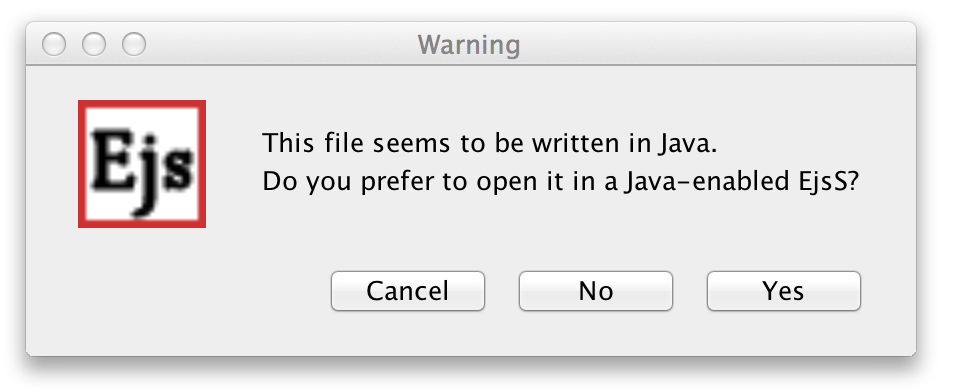
\includegraphics[scale=\scale]{04JavatoJS/images/FlavorDetection.png}
  \caption{Dialog caused by a possible programming language conflict.}
  \label{fig:04JavatoJS/FlavorDetection}
\end{figure}

\noindent The options provided by this dialog are the following:
\begin{description}
  \item[Cancel]: This will stop loading this file altogether.
  \item[No]: This will ignore the conflict and will load this file.
  \item[Yes]: This will launch a new instance of \ejs\ with the correct programming language support and will load this file in it.
\end{description}

You need to select \textbf{No} for the purposes of this chapter. This will open the original Java file in this Javascript instance of \ejs. You will notice that the \lit{Description} and \lit{Model} tabs of \ejs\ are loaded with the information of the \file{MassAndSpring.ejs} file, but the \lit{HtmlView} tab will remain empty.

Before we do any changes, and in order to preserve the original file, we want to save the file with the extension for Javascript files, \file{.ejss}. Click now the \lit{Save as} icon of \ejs' taskbar, 
\includegraphics[scale=\linescale]{../_common/icons_png/saveAsSmall.png}, (preferably) change to a different directory of your workspace \file{source} directory, and change the name of the output file to \file{MassAndSpring.ejss}. That is, just change the file  extension to \file{.ejss}. This extension identifies the new file as a Javascript \ejs\ file. 

Now, \ejs\ will proceed to save the new file and will detect that this file has a Java view and ask you whether you want to save it or not. See Figure~\ref{fig:04JavatoJS/ForgetJavaView}. 

\begin{figure}[htb]
  \centering
  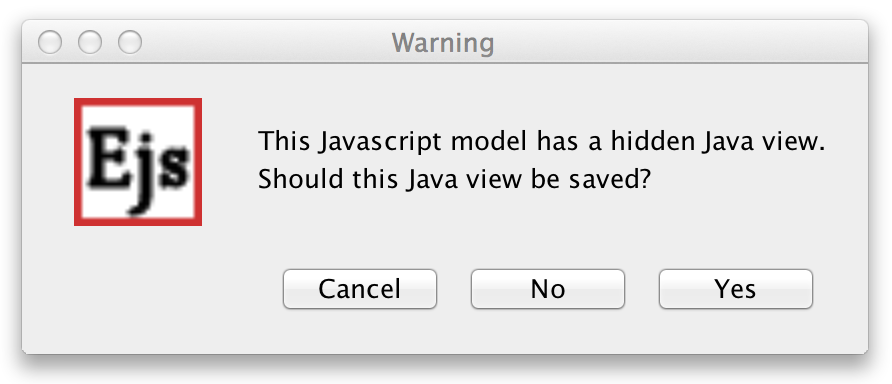
\includegraphics[scale=\scale]{04JavatoJS/images/ForgetJavaView.png}
  \caption{Dialog concerned about the existing Java view.}
  \label{fig:04JavatoJS/ForgetJavaView}
\end{figure}

\noindent Your answer should be \textbf{No}. We won't need the Java view in our new Javascript simulation. (Recall that, since we chose a different extension for the new file, the original \file{MassAndSpring.ejs} file remains unchanged.) \ejs\ will have saved the new file and, if necessary, copied any auxiliary files required by this simulation (if you changed the target directory), thus creating a completely independent new simulation file. We are now ready to start the transition to a pure Javascript simulation.

% ------------------------
    \section{Changes to the Description}\label{section:04Description}
% ------------------------

The good news for the \lit{Description} is that no changes are really needed. The Description are just HTML pages that will work just fine for the Javascript model.

If only, we recommended that you review your HTML files to make sure the HTML code in them is correctly formed. The reason is that, if you later want to create an ePUB document with your Javascript simulation, \ejs\ needs the HTML code to be correct. More precisely, ePUB documents require XHMTL files (which are basically more strictly enforced HTML files) and \ejs\ can either take XHTML files or try to convert your (correctly formed) HTML files for it.

Typical editions required to make an HTML file correct include the following:

\begin{itemize}
  \item Make sure all HTML opening tags have their corresponding closing tag. In particular, paragraphs tags $<p>$ need a matching  $</p>$.
  \item Make sure all HTML single tags have a closing $/$, as in $<br />$.
\end{itemize}
\noindent However, the best recommendation we can make to you, if you plan to create ePUB documents with your description pages in them, is that you create stand-alone valid XHTML file (you can validate them with free tools available on the Internet) and use the \lit{Description} feature that lets you link your pages to external HTML or XHTML pages (see Figure~\ref{fig:04JavatoJS/LinkHTMLPage}). 

\begin{figure}[htb]
  \centering
  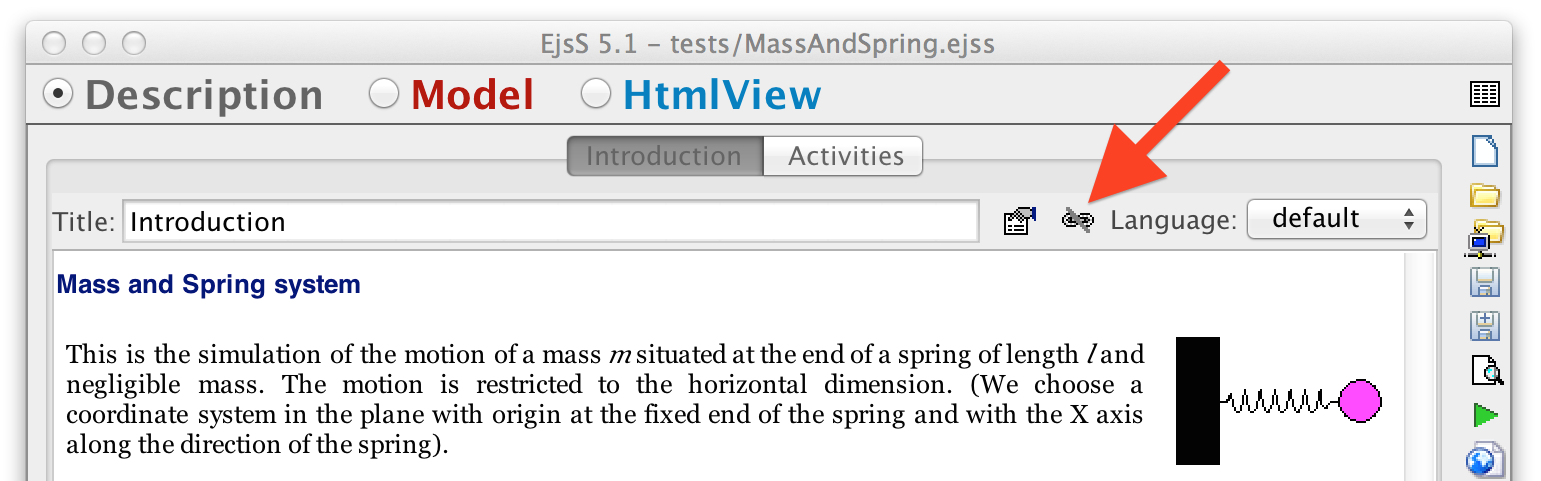
\includegraphics[scale=\scale]{04JavatoJS/images/LinkHTMLPage.png}
  \caption{Icon to link a description page to an external HTML or XHTML file.}
  \label{fig:04JavatoJS/LinkHTMLPage}
\end{figure}

% ------------------------
    \section{Changes to the Model}\label{section:04Model}
% ------------------------

The model needs that you change all Java code to Javascript code. Let's examine in detail each of the parts of the model for our sample simulation and do the required changes.

\subsection{Variables}

Javascript has no types for variables. All variables are declared with a \lit{var} keyword. This means that, in principle, Javascript makes no difference among integers, doubles, Strings, etc.\ldots But it does! For instance, you should not use a double variable as index for an array.

For this reason, and also because it helps clarify the use of variables in your model (what values they can have and where you can or cannot use them), we have left the feature that forces you to assign a type to a variable. The types accepted are the basic ones, and no more.

If, for any reason, your Java model has variables declared to be of any non standard type (java.awt.Color is a typical example of this), you must convert it to one of the predefined types. (By the way, colors are indicated in HTML5 using strings.) If your model uses sophisticated Java objects you may have created or imported from an external library, then you are in trouble. Again, you must resort to using only basic types. 

The initial values you can assign to basic variables are very much like what you can assign them in Java. (Arrays an objects are an exception, see below.) For this reason, simple models do not require \emph{any} change at all in the tables of variables, when changing them from Java to Javascript. 
In particular, our example needs no change to the \lit{Variables} part of the model.

\subsubsection*{Arrays}

Arrays are declared somewhat differently in Javascript. The editor for variables in \ejs\ takes care of this and you need only to indicate the dimensions, as you would do in the Java flavor. However, giving an initial value to an array is different, since Javascript uses square brackets as delimiters in an array, while Java uses braces. Hence, an initial value like this in Java:
\begin{verbatim}
double[][] myArray = new double { {1.0,2.0,3.0}, {3.0,4.0,5.0} };
\end{verbatim}
\noindent should be written as follows in Javascript:
\begin{verbatim}
var myArray = [ [1.0,2.0,3.0], [3.0,4.0,5.0]];
\end{verbatim}
Also, resizing an array is different in Javascript. The Java syntax:
\begin{verbatim}
doubleArray = new double[n][m];
\end{verbatim}
\noindent converts in Javascript to:
\begin{verbatim}
doubleArray = new Array(n);
for (var i=0; i<n; i++) doubleArray[i] = new Array(m);
\end{verbatim}
\noindent (assuming \verb?n? and \verb?m? are valid integers). A final difference is that Javascript does not guarantees to initialize to 0 the elements of the allocated array, nor check for incorrect use of indexes.

\subsubsection*{Objects}

Javascript supports the concept of an \lit{Object}. Basic objects are just dictionaries of other variables. You add variables to objects as follows:
\begin{verbatim}
var myObject  = { };
myObject.name = "My object";
myObject.value = 3.0;
\end{verbatim}
\noindent The use you make of these variables is up to you. Sophisticated use of Javascript objects is allowed, though out of the scope of this manual.

\subsubsection*{Variables not declared}

Finally, Javascript is a loose language and does not force you to declare variables before using them. For instance, the code
\begin{verbatim}
n = 3;
_println ("n = "+n);
\end{verbatim}
\noindent will produce the intended result, even if \verb?n? has not been declared elsewhere. This may lead to undesired results, if you happen to type incorrectly one of your variables. (Javascript will think it is a new one!) Watch for this caveat. \ejs\ tries to help you with this problem and incorporates a \lit{Lint} processor~\footnote{\link{http://en.wikipedia.org/wiki/Lint\_(software)}} that looks for potential errors in your code, including this one. In occasions like the one described here, the \ejs\ \lit{Output area} will display a message like the following, when you try to run the simulation:
\begin{verbatim}
Lint error: 'n' is not defined.
     n=3;   // > Initialization.Init Page:1
\end{verbatim}

\subsection{Pages of code}

All pages of code in the \lit{Initialization}, \lit{Evolution}, \lit{Fixed relations} and \lit{Custom} must be changed from Java to Javascript syntax. Fortunately, the syntax of algorithms for both programming languages is very similar. The main changes usually required for code in these parts of the model are the following:
\begin{itemize}
  \item Use \verb?var? to declare local variables, instead of \verb?int?, \verb?double?, etc. A typical place for this is in \verb?for? loops.
  \item The scope of local variables is that of the block in which they are used. Even if you declare them \emph{after} they are used. For this reason, it is recommended to declare all variables for once at the beginning of each page of code.
  \item Function declaration in Javascript includes no information about the return type or the type of the parameters. A declaration of a Java function like this:
\begin{verbatim}
public double force (double time) {
  return amp*Math.sin(freq*time); 
}
\end{verbatim}
\noindent turns into the following Javascript code:
\begin{verbatim}
function force (time) {
  return amp*Math.sin(freq*time); 
}
\end{verbatim}
\end{itemize}

Our sample simulation requires no change of its \lit{Fixed relations} page of code, since the Java expressions:
\begin{verbatim}
T = 0.5*m*vx*vx;
V = 0.5*k*(x-L)*(x-L);
E = T + V;
\end{verbatim}
\noindent are also valid Javascript expressions.

\subsubsection*{ODE editor}

The use of the ODE editor, for evolution pages that require solving ordinary differential equations, is straightforward. The only obvious change is that expressions in the rate equations and code in preliminary code, events, and other pages of code, need to use valid Javascript syntax. The Javascript ODE editor implements, for the time being, less solvers than its Java counterpart. But the underlying code and mechanisms are exactly the same.

\subsection{Model elements}

The Javascript flavor of \ejs\ includes also the concept of \lit{Model elements}, as a way to access third party Javascript libraries. However, the elements provided by the Java and Javascript flavors are completely different and there is no attempt to make this implementation converge.

Model elements used by your simulation, should your original Java simulation use them, are preserved to make you conscious of their need for your model. But you must immediately remove them and replace them by equivalent Javascript model elements, or by your own coding. 

In other words, porting from Java to Javascript (or viceversa) simulations that depend on the use of Model elements can be extremely difficult.

% ------------------------
    \section{Implementing an HTML View}\label{section:04View}
% ------------------------

One part of the simulation that needs to be completely created from scratch is the \lit{HtmlView}. The reason is that creating graphical user interfaces with Swing (the Java library for interfaces) and HTML5 is based on completely different principles. To name one, Swing is a window-oriented platform, while HTML5 is designed to be displayed inside a web browser in a single window.

For this reason, we decided to create a number of pure HTML5 elements, based on our past experience with Java, but adopting a newer approach, more natural to HTML5 and not restricted by backwards compatibility issues. The result is a collection of HtmlView elements that you combine (in a similar way to how you combined View elements) to create interfaces of great quality and with the same flexibility as with the Java version.

An important difference with the Java flavor is that a simulation can have more than one HtmlViews. Although many authors typically only create one, we have provided this feature for situations where you want to plan to support devices with different sizes and orientations. Each HtmlView you create has a preferred with and height that you specify. In runtime, if you provided more than one HtmlViews, the simulation will use the one that best matches the device' screen size and orientation.

In our case, we will create only one HtmlView that resembles the one of the original Java version. So, click on the empty HtmlView panel to create an initially empty HtmlView. 

Now, it is a very good idea to launch a Java flavored instance of \ejs\ and load into it the original \file{MassAndSpring.ejs} file. The reason is that we want to have both instances of \ejs, the Java and the Javascript flavors, side by side, and inspect the Tree of View elements in the former, as we create and customise the Tree of HtmlView elements in the latter. Figure~\ref{fig:04JavatoJS/ViewsSideBySide} shows both views (the Javascript HtmlView still empty), side by side. 

\begin{figure}[htb]
  \centering
    \subfigure{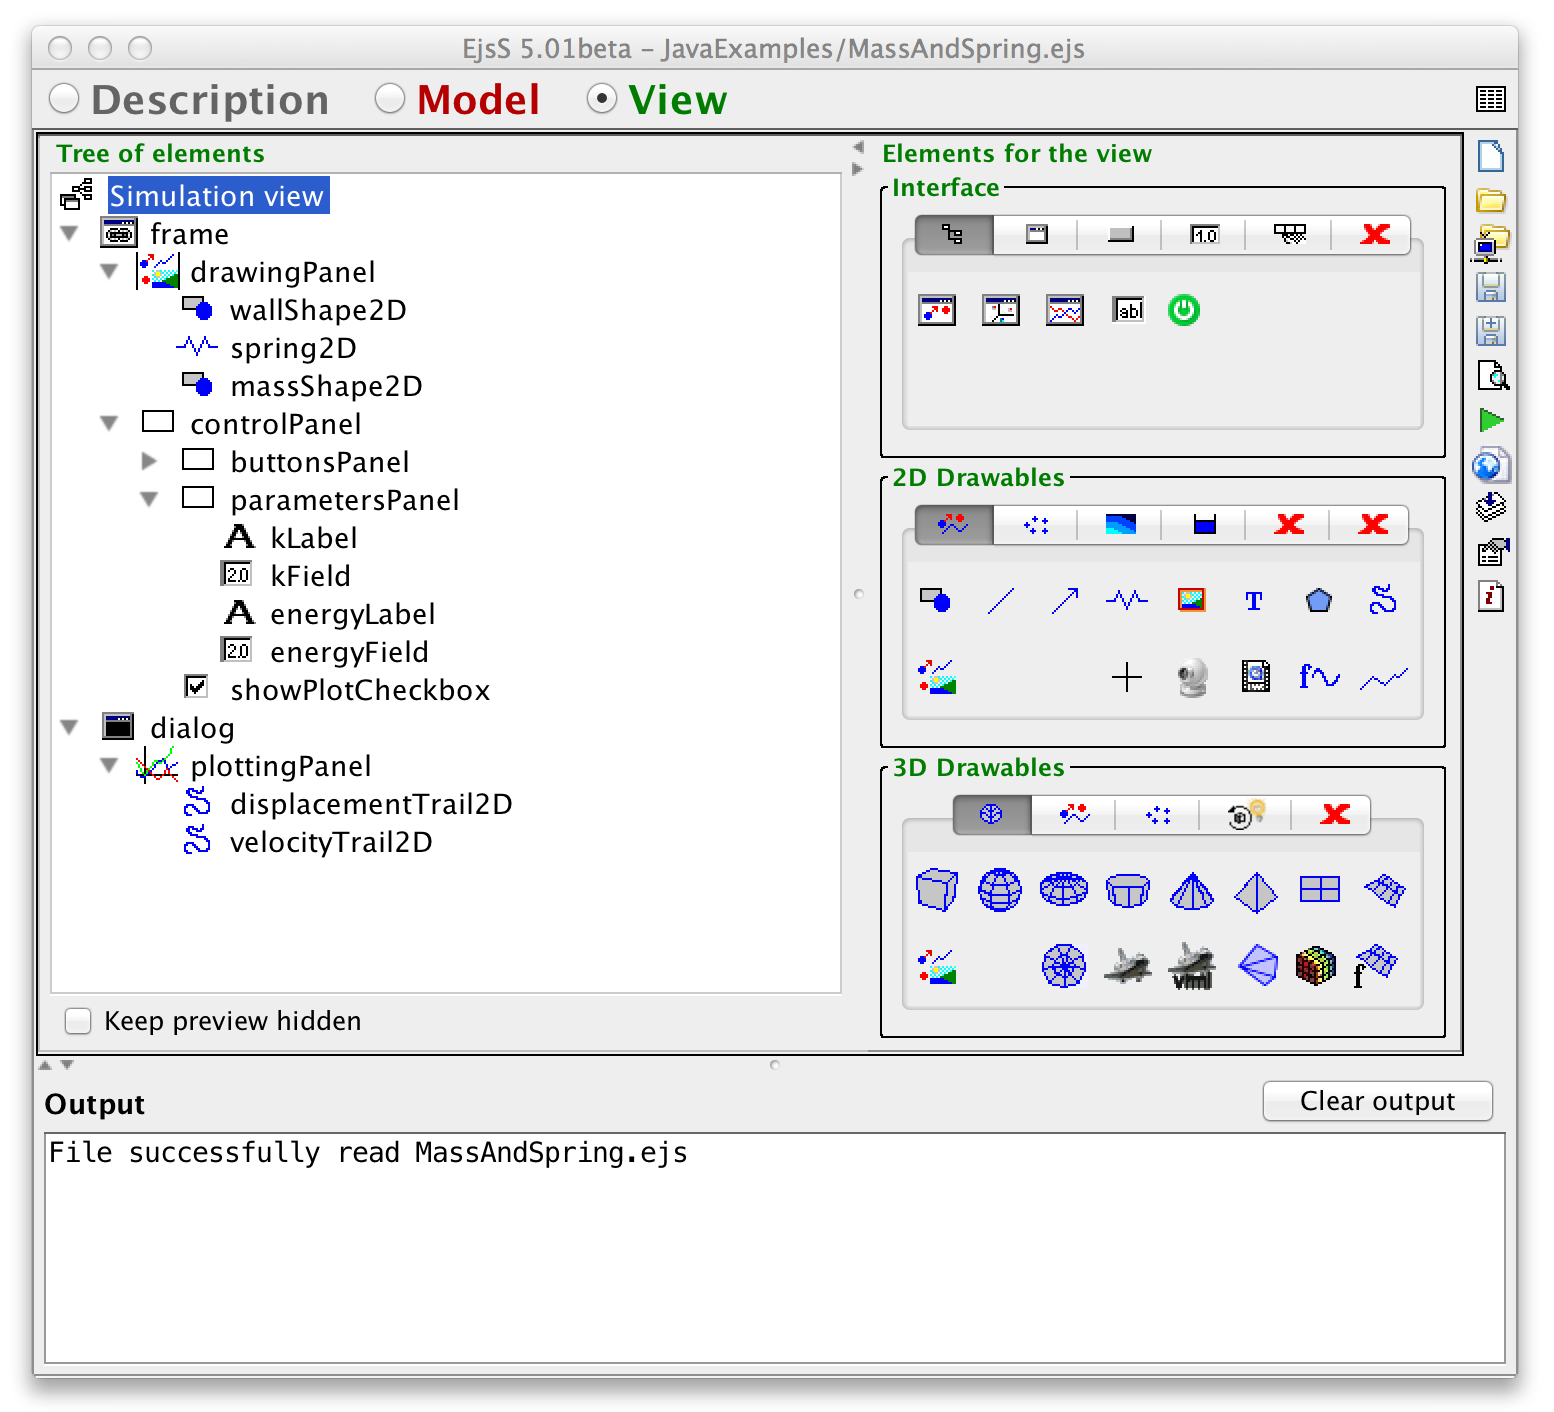
\includegraphics[scale=0.2]{04JavatoJS/images/JavaView.png}}
    \subfigure{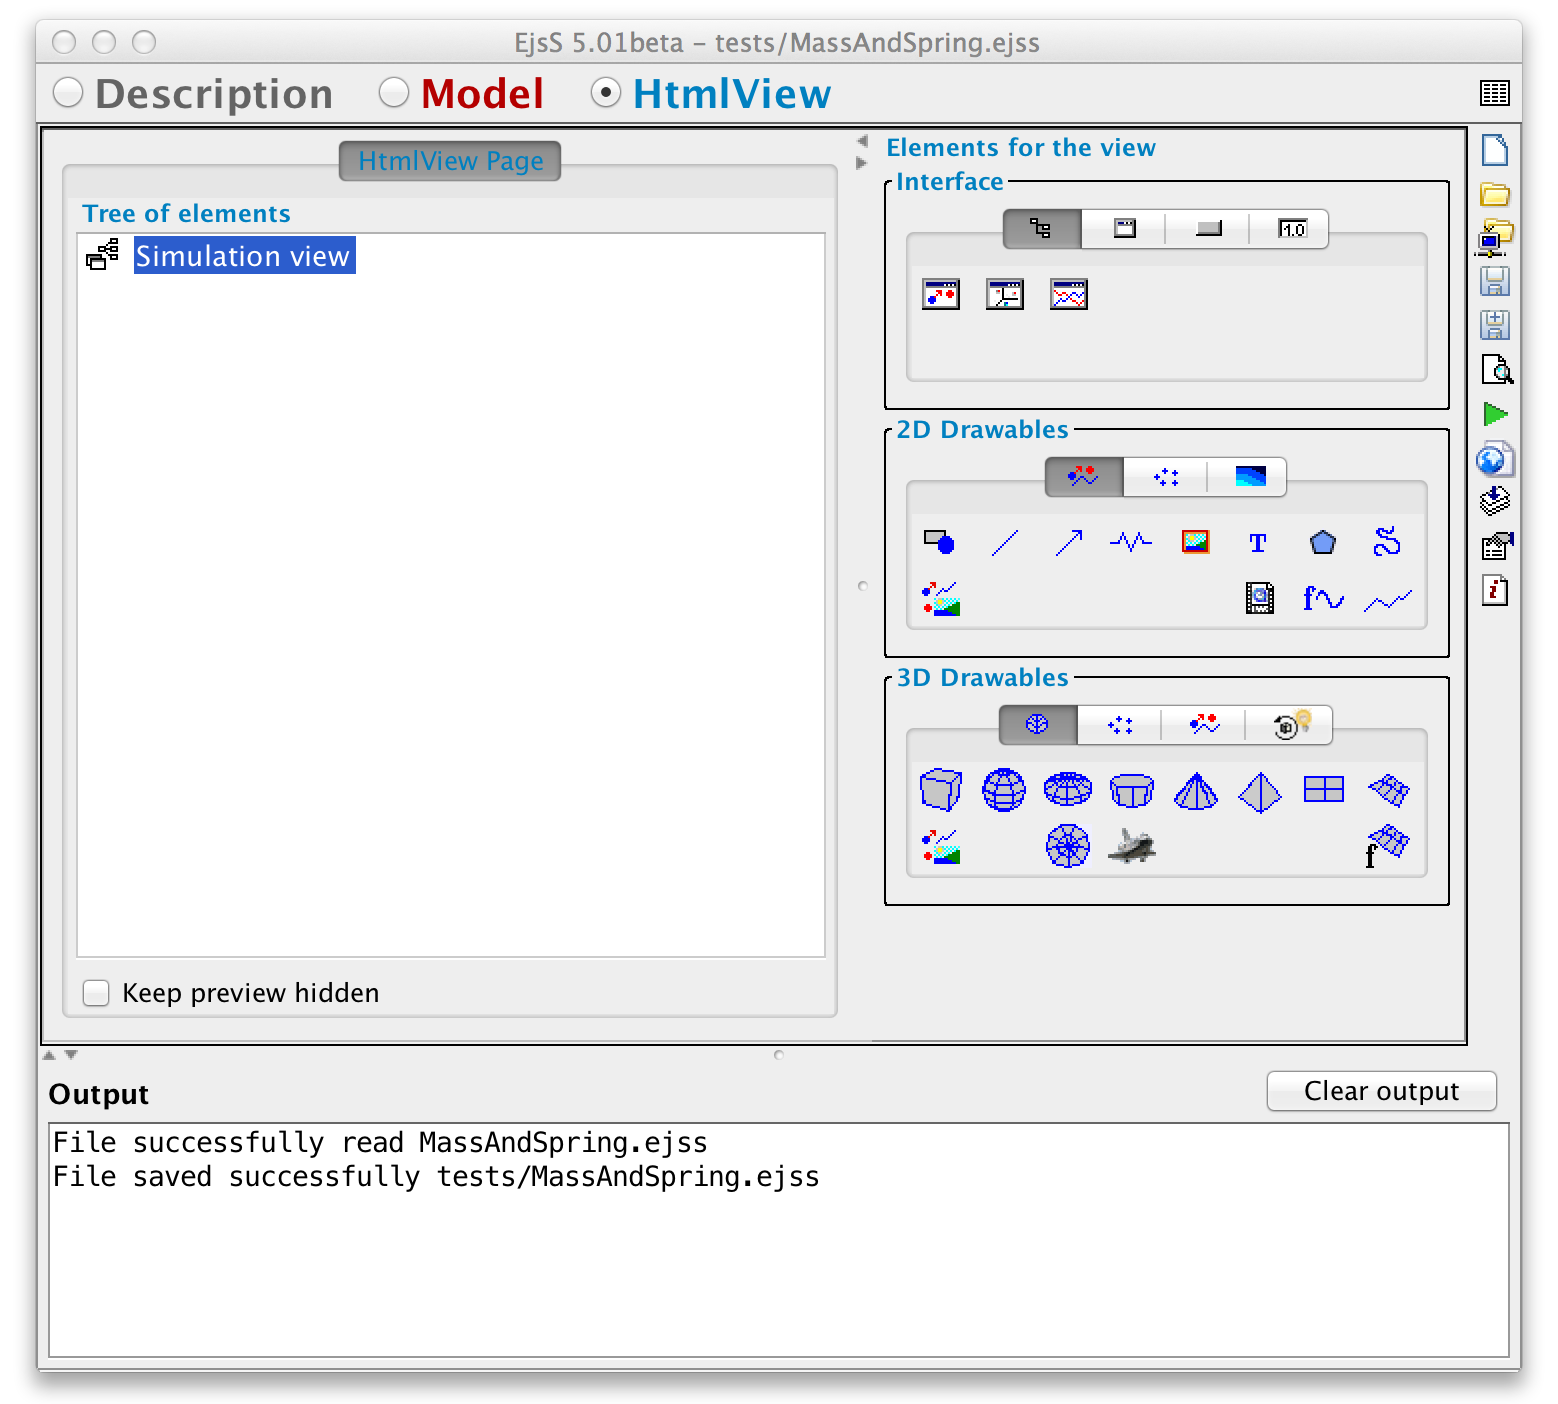
\includegraphics[scale=0.2]{04JavatoJS/images/JavascriptView.png}}
  \caption{Java tree of elements (left) and empty HTML5 tree of elements.}
  \label{fig:04JavatoJS/ViewsSideBySide}
\end{figure}

Your task consists now of creating the HtmlView by selecting the elements provided by the HtmlView palette, in a way that mimics the selection done by the Java version. You will need to customise each HtmlView element's properties to match the use of the model variables and actions that was done in the original Java view. (Recall to write valid Javascript code for the action properties!)

A good way to speed up the process is to make use of Custom elements (provided in the first tab of the \lit{Interface} palette. These consist of a selection of predefined combinations of HtmlView elements that are common to many simulations.

The creation of a new HtmlView, element by element, is, perhaps, the most time-consuming part of the process of porting an existing Java simulation to Javascript. We don' t get into details here, but you can see the final result of our work in the \file{JavascriptExamples/MassAndSpring.ejss} file included in your workspace by the standard distribution of \ejs.

One important feature of HtmlView interface elements is the presence of a \lit{CSS} property. This property lets you set directly the CSS characteristics of the underlying HTML5 element. CSS (Cascading style sheets) is a complex and flexible environment to help create very nice interfaces, and we do not try to cover it here. But any knowledge of CSS will help you improve your HtmlViews. ~\footnote{See for instance \link{http://www.w3schools.com/css/}.}

Another feature of the implementation of HtmlView element properties is that you can very easily set any of them programatically. Just use a sentence of the form:
\begin{verbatim}
_view.elementName.setProperty("PropertyName",value);
\end{verbatim}
\noindent where \verb?elementName? is the name you gave to the element, \verb?PropertyName? is the name of the property as it appears in the property edition dialog, and \verb?value? is the value you want to give to the property. Examples of this are:
\begin{verbatim}
_view.plottingPanel.setProperty("Display","none"); // Hide it
_view.bottomPanel.setProperty("Width",450); // Resize it
\end{verbatim}

% ------------------------
    \section{Conclusion}\label{section:04Conclusion}
% ------------------------

As conclusion for this chapter, we just repeat what we said at its beginning. Porting an existing Java simulation to a pure Javascript one is rather straightforward in \ejs, and consists of the following steps:

\begin{numberlist}

  \item Loading the \file{.ejs} file and saving it as a \file{.ejss} file.
  \item Review the \lit{Description} pages for HTML correctness.
  \item Edit the Java code in different editors of the \lit{Model} to convert it to equivalent Javascript code. 
  \item Create a HTML-based \lit{HtmlView} that mimics the original Java based \lit{View}.   
\end{numberlist}

\noindent Creating the HtmlView is, by far, the most time-consuming part of the process.





